\section{Diskussion}
\label{sec:Diskussion}

Die Kennlinien lassen für Heizströme bis $I_\text{H} = 2,3\,\si{\ampere}$ eine gute Bestimmung der
Sättigungsströme zu. Bei höherer Heizstromstärke lässt die Genauigkeit allerdings nach, da die aufbaubedingt
maximal mögliche Beschleunigungsspannung bereits ausgeschöpft ist.

\noindent Zur Verifizierung des Langmuir-Schottkyschen Raumladungsgesetztes wird der per Ausgleichsrechnung bestimmte
Exponent $a = (1,12 \pm 0,03)$ mit dem zu erwartenden Exponenten $a_\text{Theorie} = 1,5$ verglichen. Es ergibt sich eine relative
Abweichung von $25,33\,\%$. Diese lässt sich durch die geringe Anzahl der zur Auswertung nützlichen Messwerte begründen,
da das Raumladungsgebiet im Graphen verhältnismäßig klein ausfällt, was sich durch eine höhere Heizstromstärke verbessern ließe.

\noindent Bei der Untersuchung des Anlaufstromgebiets wird die Kathodentemperatur bestimmt. 
Diese wird mit der über die Leistungsbilanz des Heizstromkreises bestimmten Kathodentemperatur verglichen.
Die Abweichung der Ergebnisse der beiden Messmethoden für die Temperatur der Kathode liegt bei 17,94 bzw. 21,86\,\%,
wobei anzumerken ist, dass nicht eindeutig ist, welcher der tatsächlichen Temperatur näher liegt.

\noindent Bei einem Vergleich der bestimmten Austrittsarbeit $W = (4,65 \pm 0,08)\,\si{\eV}$ mit dem Theoriewert
für Wolfram $W_\text{Wolfram} = 4,54\,\si{\eV}$ \cite{kent2} ergibt sich eine relative Abweichung von $2,37\,\%$. Trotz der
geringen Abweichung, welche sich durch die Abschätzung der Sättigungsströme erklären lässt,
lässt sich die Theorie hierbei bestätigen. 

\section{Anhang}
\label{Anhang}
Im folgenden sind die Kopien der Messwerte aufgelistet.

\begin{figure}[H]
  \centering
  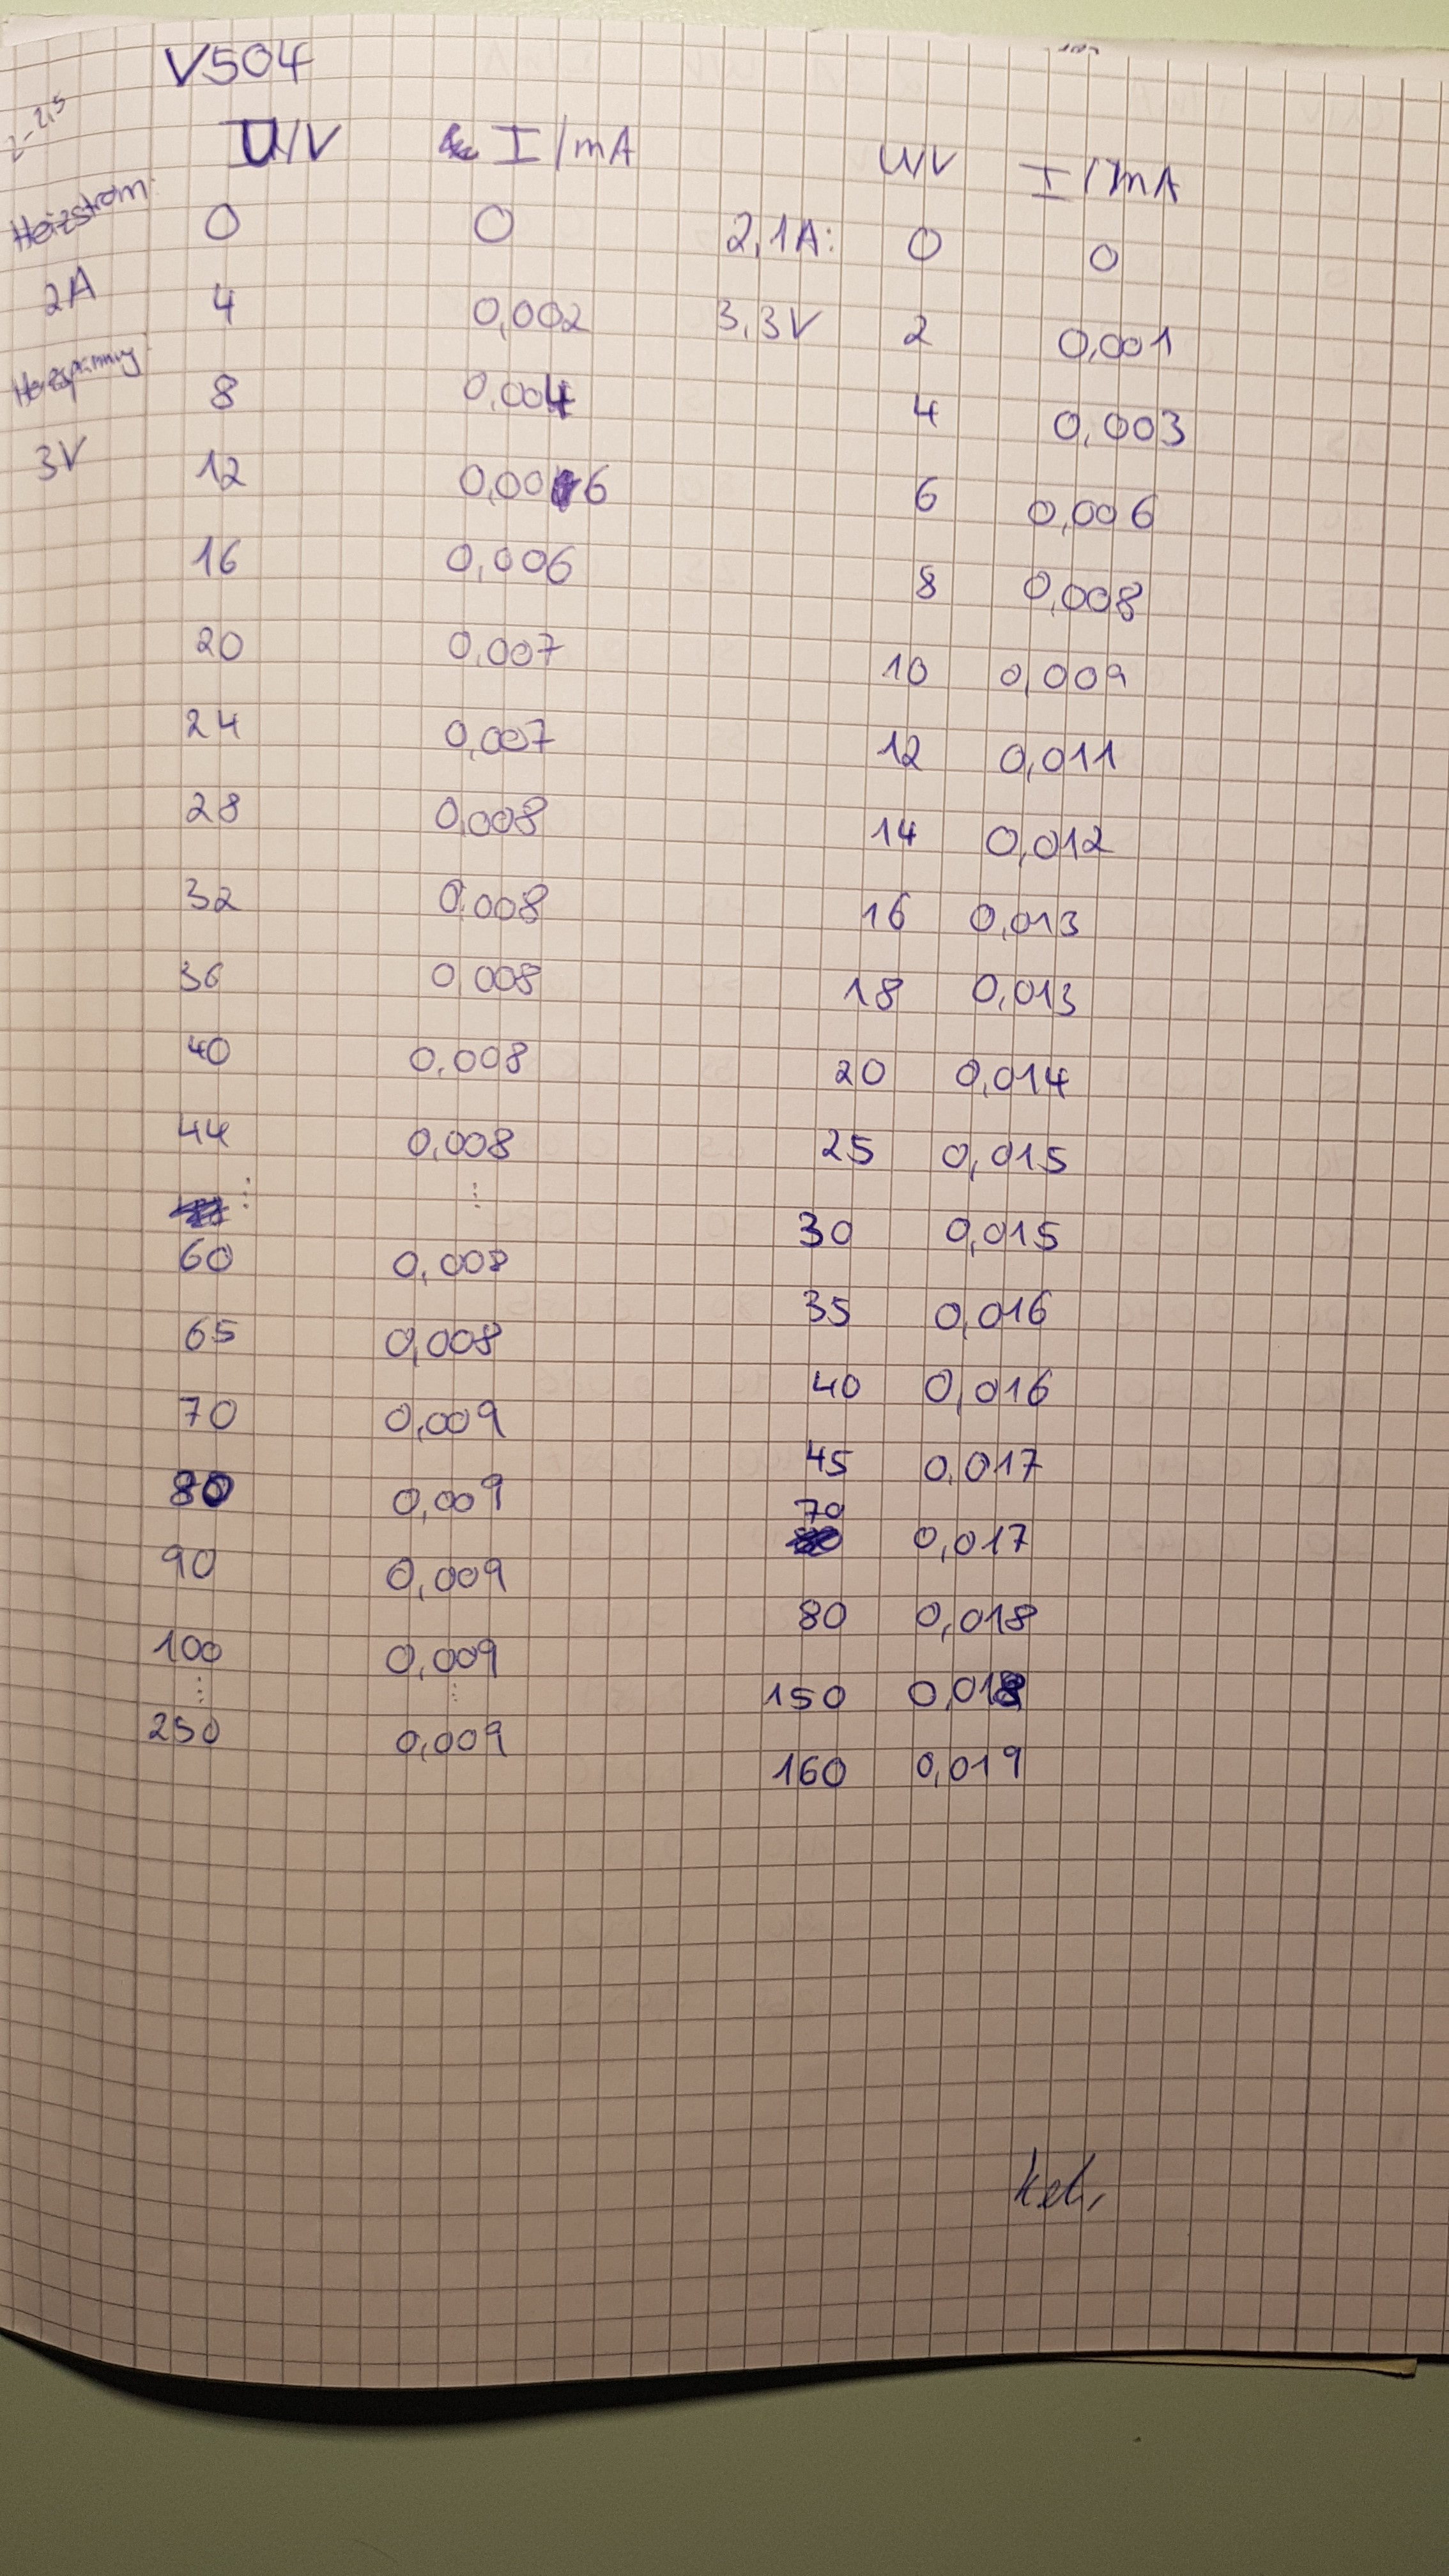
\includegraphics[height=24cm]{Messung (1).jpg}
\end{figure}

\begin{figure}[H]
  \centering
  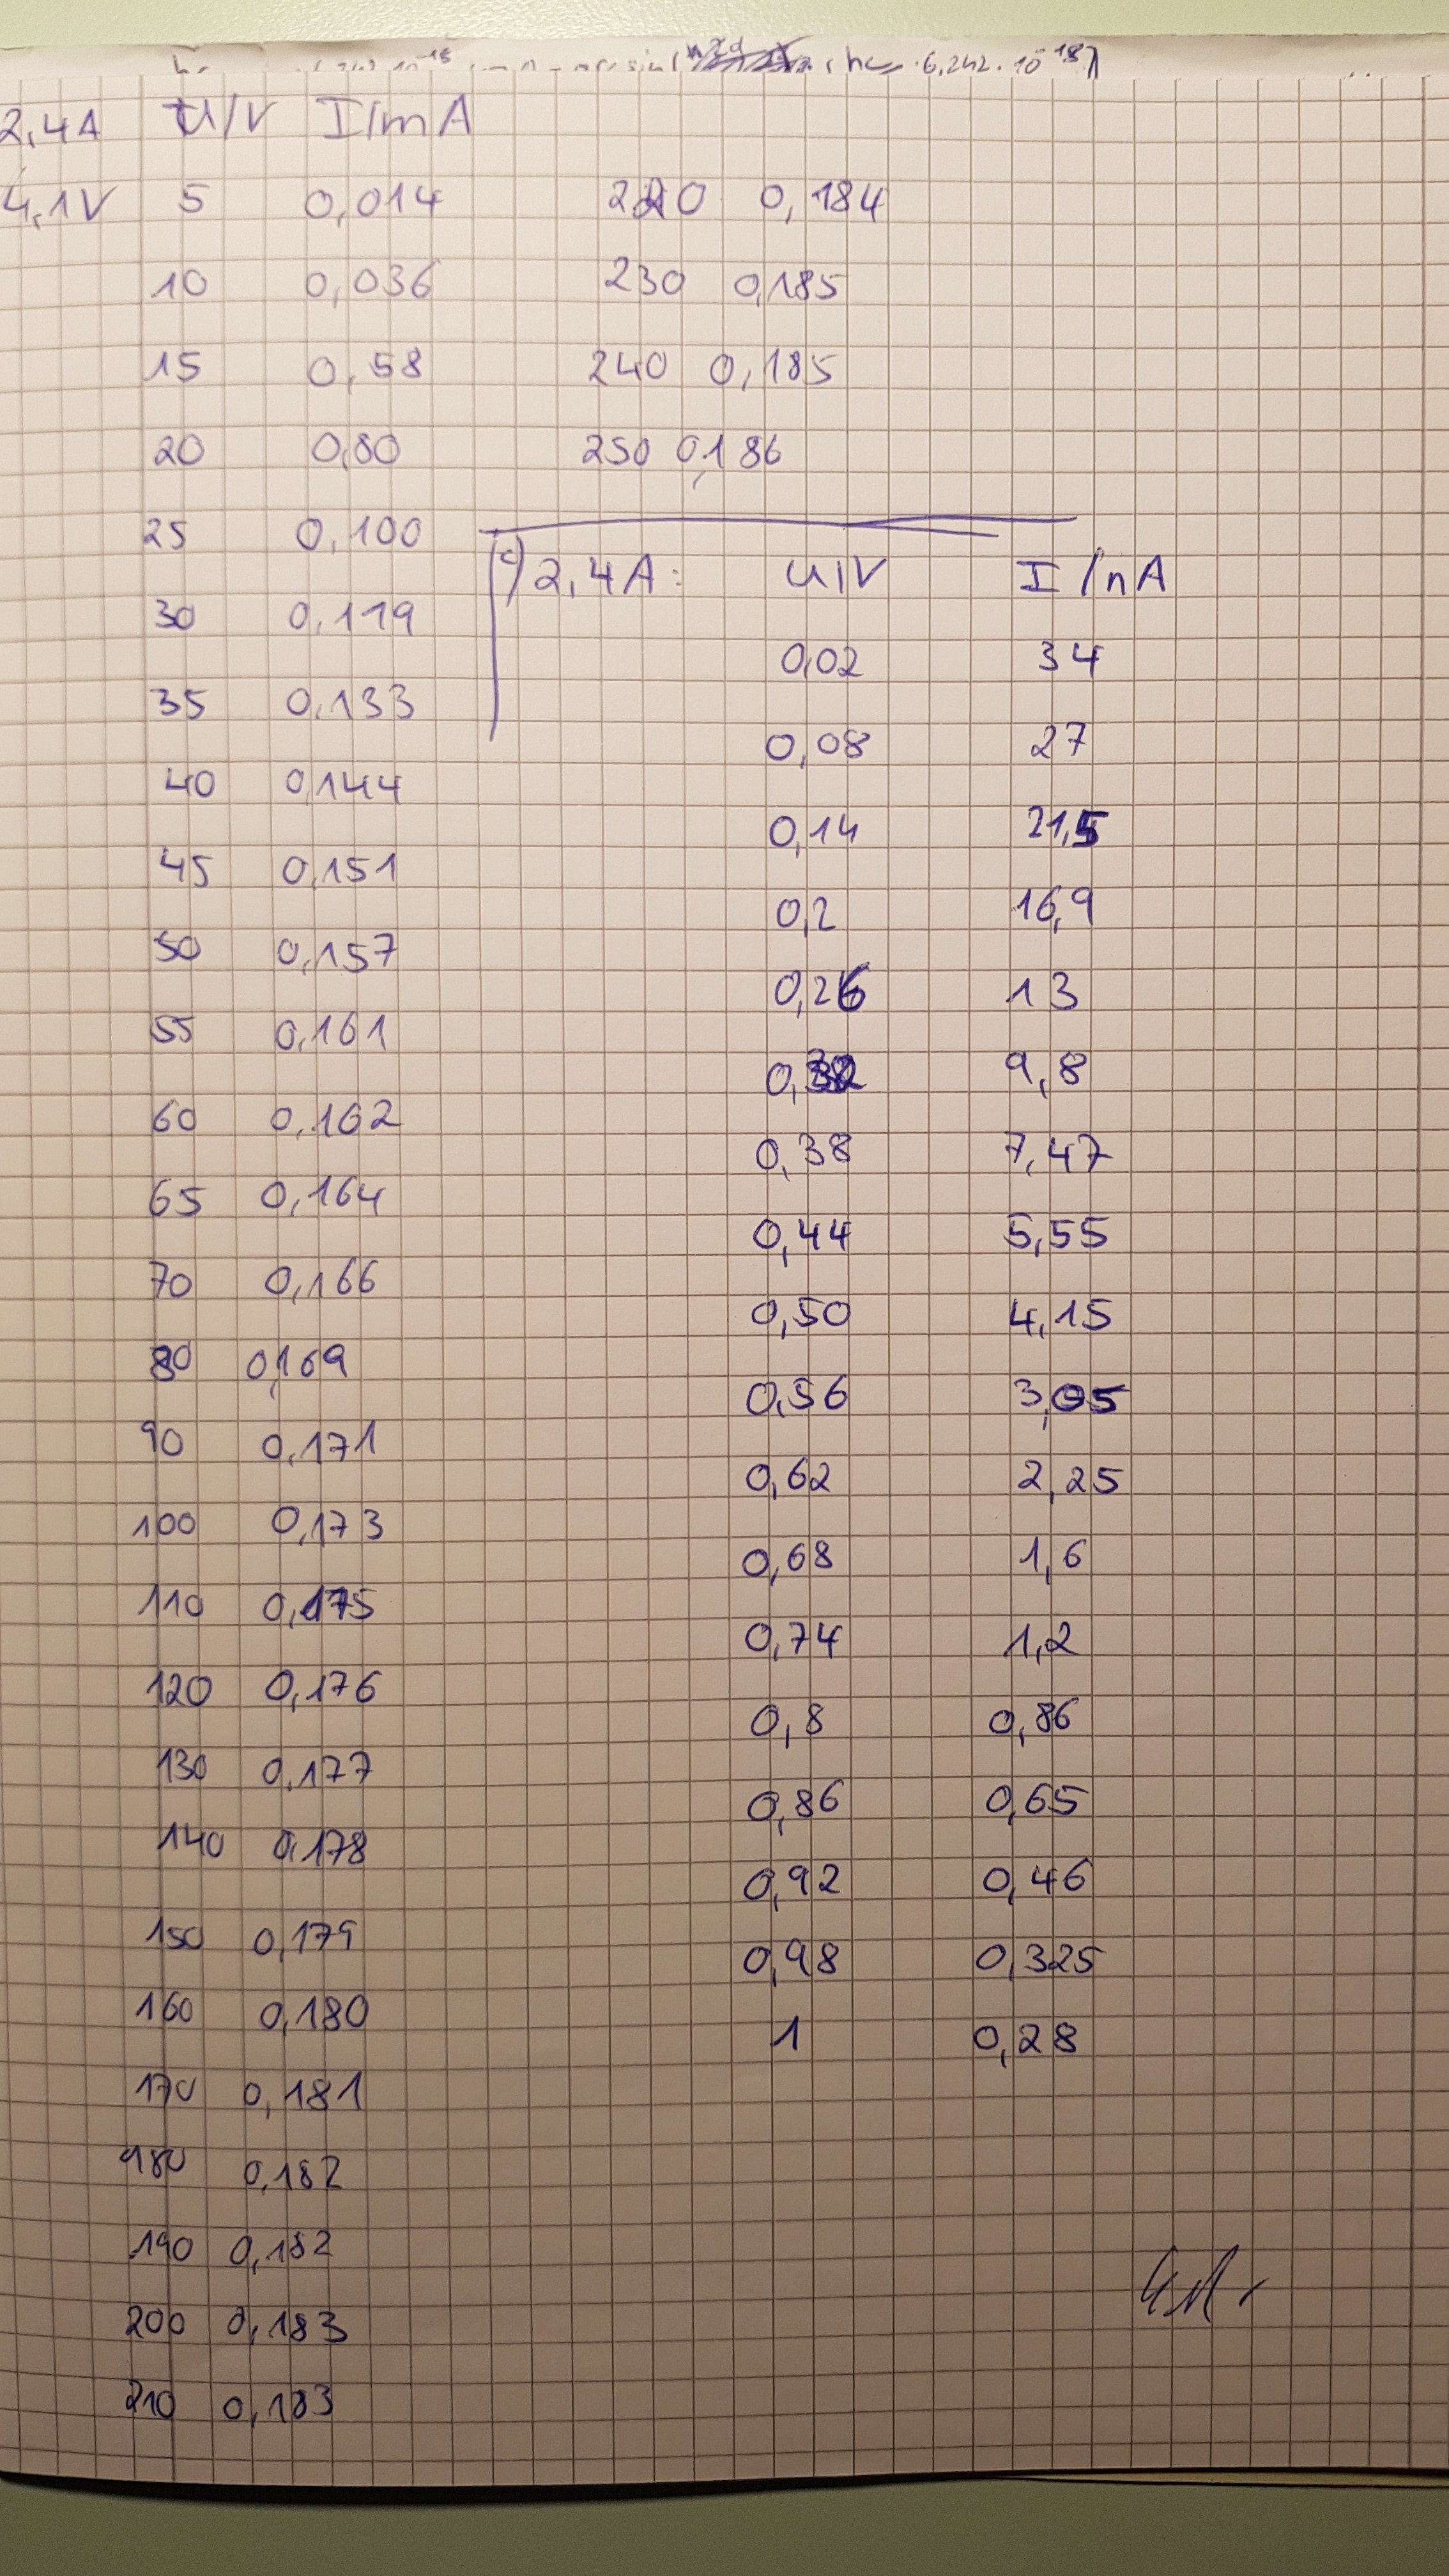
\includegraphics[height=24cm]{Messung (2).jpg}
\end{figure}

\begin{figure}[H]
  \centering
  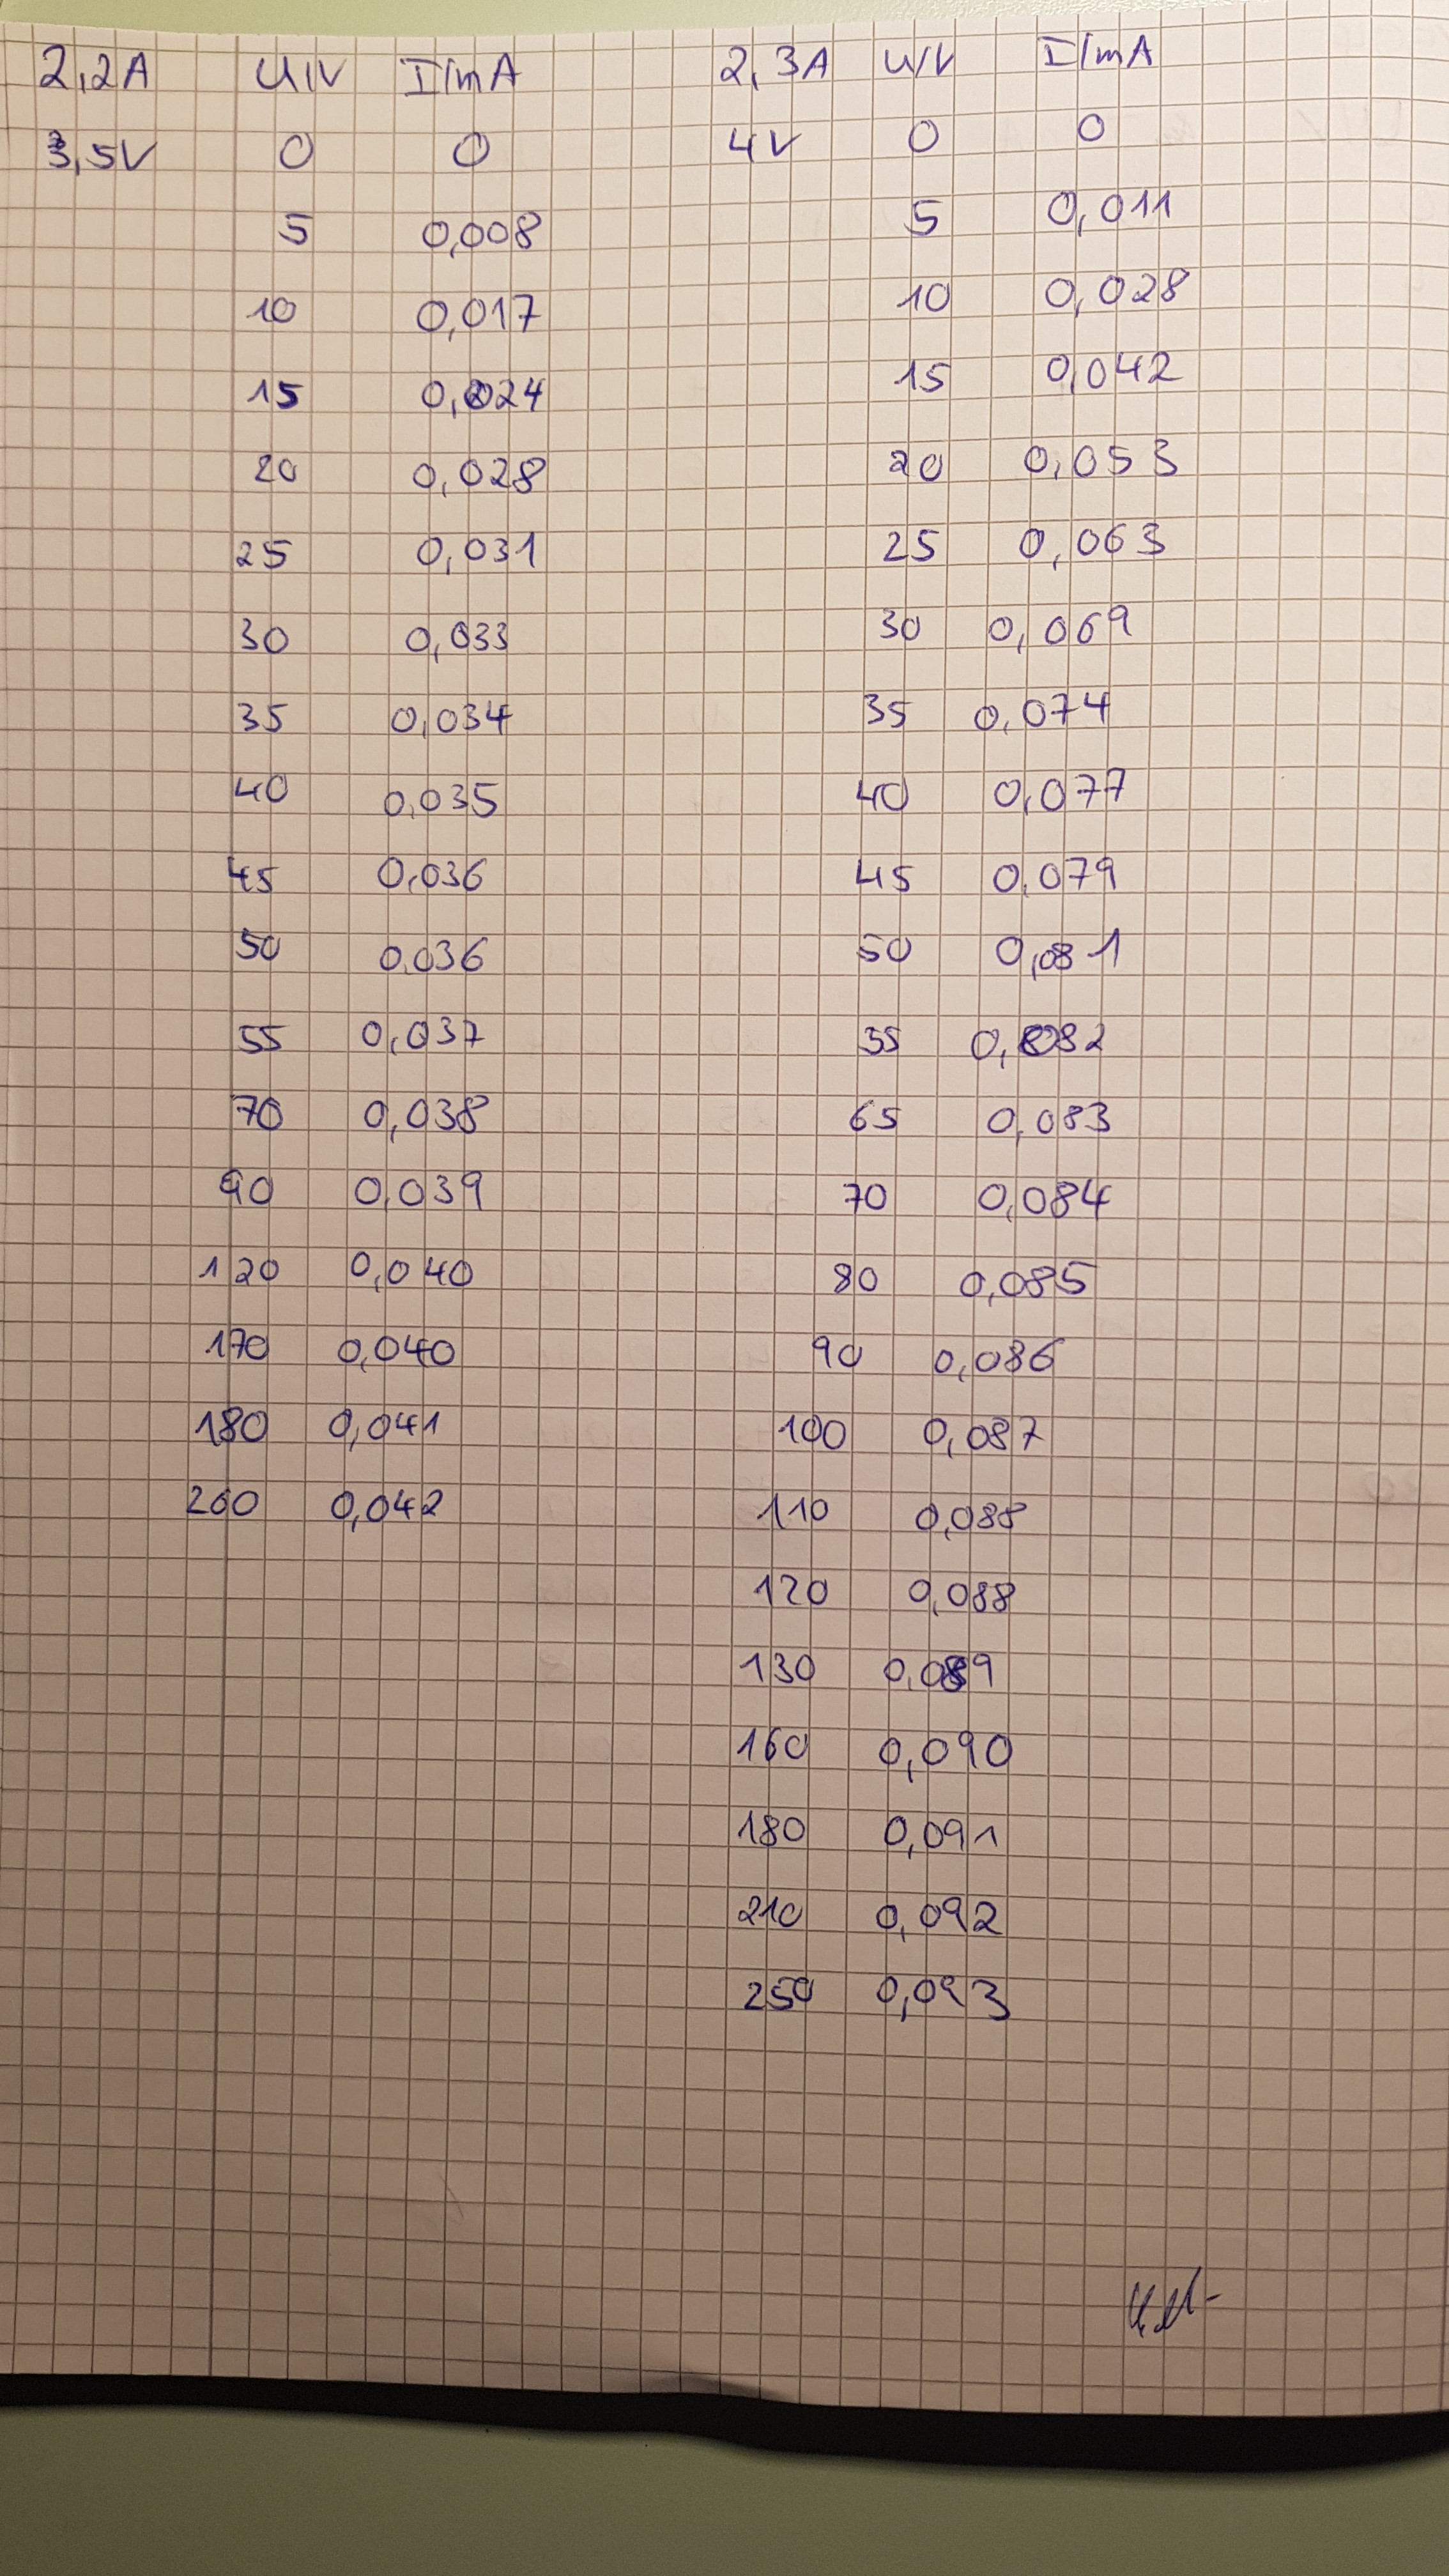
\includegraphics[height=24cm]{Messung (3).jpg}
\end{figure}
